\begin{frame}
\frametitle{Assumptions}
\begin{columns}
	\begin{column}{.55\textwidth}
		\begin{block}{Cyclus Requirements} 
			\begin{itemize}
				\item Modular.
				\item Time step $\geq$ 1 month
				\item Streams must be in a
				trade-able form.
				\item Parameters are constant for the simulation.
				\begin{itemize}
					\item Equation input toolkit under development.
				\end{itemize}
				\item Diversion detection must be added after.
			\end{itemize}
		\end{block}
	\end{column}
	\begin{column}{.45\textwidth}
		\begin{figure}
			\centering
			
\includegraphics[width=0.9\linewidth]{cyclus}
			\label{fig:cyclus}
		\end{figure}
	\end{column}
\end{columns} 
\end{frame}

\begin{frame}
\frametitle{Subprocesses - Voloxidation}
		\begin{figure} 
			\centering
			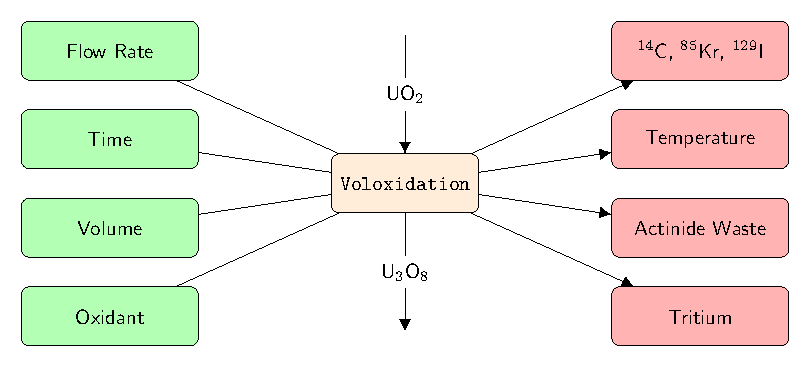
\includegraphics[width=0.9\linewidth]{volox}
			\caption{Voloxidation material balance area \cite{jubin_spent_2009}.}
			\label{fig:volox}
		\end{figure}
\end{frame}
\begin{frame}
\frametitle{Subprocesses - Electroreduction}
		\begin{figure} 
			\centering
			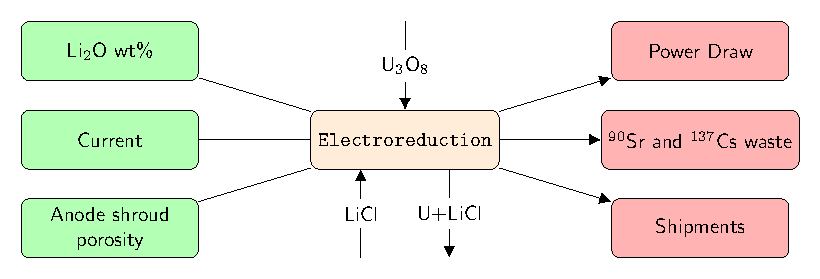
\includegraphics[width=0.9\linewidth]{reduction}
			\caption{Reduction material balance area \cite{lee_advanced_2008}.}
			\label{fig:reduction}
		\end{figure}
\end{frame}
\begin{frame}
\frametitle{Subprocesses - Electrorefining}
		\begin{figure}
			\centering
			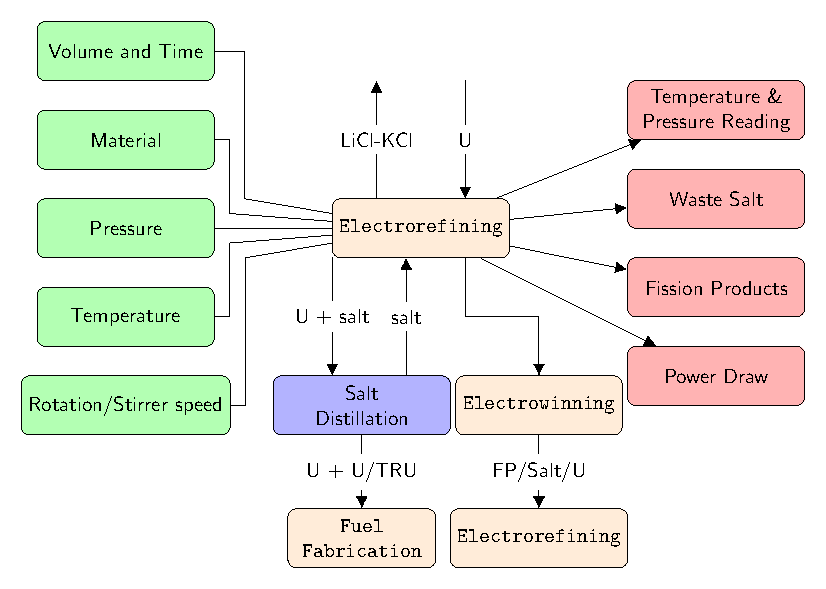
\includegraphics[width=0.85\linewidth]{refining}
			\caption{Refining material balance area \cite{lee_advanced_2008}.}
			\label{fig:refining}
		\end{figure}
\end{frame}
\begin{frame}
\frametitle{Subprocesses - Electrowinning}
		\begin{figure} 
			\centering
			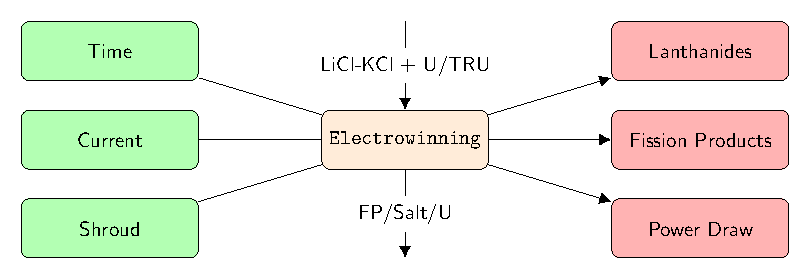
\includegraphics[width=0.8\linewidth]{winning}
			\caption{Winning material balance area.}
			\label{fig:winning}
		\end{figure}
\end{frame}